%Template pembuatan proposal skripsi.
\documentclass{jtetiproposalskripsi}

%-----------------------------------------------------------------
%Disini awal masukan untuk data proposal skripsi
%-----------------------------------------------------------------
\titleind{TEKNIK KRIPTOGRAFI UNTUK MENGAMANKAN INFORMASI DENGAN MEMANFAATKAN CITRA DIGITAL SEBAGAI KUNCI}

\fullname{MUHAMAD ARFIQ KHOIRON}

\idnum{1110651034}

\approvaldate{20 Desember 2014}

\degree{Sarjana Komputer}

\yearsubmit{2014}

\program{Teknik Informatika}

\headprogram{Sarjiya, S.T., M.T., Ph.D.}

\dept{Teknik}

\firstsupervisor{Ari Eko Wardoyo, S.T., M.Kom}
\firstnip{1975 0214 2005 01 1 001}

\secondsupervisor{}
\secondnip{}


%-----------------------------------------------------------------
%Disini akhir masukan untuk data proposal skripsi
%-----------------------------------------------------------------

\begin{document}

\cover

\approvalpage

%-----------------------------------------------------------------
%Disini akhir masukan untuk muka skripsi
%-----------------------------------------------------------------

%-----------------------------------------------------------------
%Disini awal masukan Intisari
%-----------------------------------------------------------------
\begin{abstractind}
Keamanan sebuah informasi kini menjadi hal yang sangat mutlak untuk menjaga agar informasi tersampaikan pada pihak yang tepat. Kriptografi merupakan ilmu untuk menyamarkan suatu pesan demi menjaga kerahasiaannya. Suatu pesan \emph{plaintext} harus melalui proses enkripsi terlebih dulu menjadi bentuk yang tidak berarti \emph{ciphertext} sebelum dikirimkan ke penerima yang berhak. Hanya pihak yang berhak lah yang dapat melakukan proses dekripsi, yaitu mengubah kembali \emph{ciphertext} menjadi \emph{plaintext} memakai suatu kunci rahasia.

Desain sebuah algoritma untuk kriptografi telah banyak dibuat oleh kriptografer, dari algoritma yang bersifat klasik maupun modern. Pada umumnya algoritma yang dibuat terkuncikan oleh sebuah teks rahasia. Pada kesempatan ini penulis akan mengembangkan algoritma \emph{caesar cipher} yang mana kunci untuk proses enkripsi dan dekripsi adalah sebuah gambar yang sama dengan memanfaatkan citra digital. Dalam sebuah citra berwarna, setiap piksel memiliki nilai intensitas warna \emph{red, green, blue} yang dapat diubah dalam sebuah data teks.

Nilai intensitas warna inilah yang akan menentukan banyaknya pergeseran huruf untuk proses enkripsi dan deskripsi yang berbeda pada tiap karakter. 
Hasil yang didapatkan adalah sebuah pengembangan dari algoritma \emph{caesar cipher} yang menggunakan citra digital sebagai kunci untuk proses enkripsi dan deskripsi. Dengan demikian informasi dalam bentuk \emph{chiphertext} akan lebih sulit dipecahkan oleh penerima yang tidak berhak.



\bigskip
\textbf{Kata kunci} : \emph{Kriptografi}, \emph{Citra Digital}, \emph{Caesar Cipher}
\end{abstractind}
%-----------------------------------------------------------------
%Disini akhir masukan Intisari
%-----------------------------------------------------------------

\tableofcontents
\addcontentsline{toc}{chapter}{DAFTAR ISI}
\selectlanguage{bahasa}\clearpage\pagenumbering{arabic}\setcounter{page}{1}

%-----------------------------------------------------------------
%Disini awal masukan untuk Bab
%-----------------------------------------------------------------
\chapter{LATAR BELAKANG}

\section{Latar Belakang Masalah}
Informasi kini menjadi sebuah kunci utama dalam segala hal. Pada masa lampau, penguasa dunia adalah dia yang memiliki pasukan yang banyak. Adanya teknologi membuat pasukan yang banyak tak lagi menguasai dunia. Pada era sekarang ini penguasa dunia adalah dia yang menguasai informasi. Barang siapa yang dapat menguasai semua informasi, maka ia dapat menguasai dunia.

Dikarenakan pentingnya informasi, berbagai cara digunakan untuk mengamankan informasi yang dimiliki agar tidak jatuh pada pihak yang tidak memiliki hak untuk mengetahui informasi tersebut. Informasi dalam bentuk teks dapat disandikan menjadi informasi lain yang tidak jelas dengan teknik kriptografi. Kriptografi merupakan ilmu yang mempelajari teknik matematis yang berhubungan dengan aspek keamanan informasi seperti keabsahan, integritas data, serta autentifikasi data (Wahana Komputer, 2010). 

Salah satu algoritma kriptografi klasik adalah \emph{Caesar cipher}, yang mana algoritma ini bekerja dengan menggeser tiga abjad ke kanan untuk setiap karakter pada deret huruf alfabet. Algoritma ini digunakan pada zaman romawi untuk menyandikan pesan yang akan disampaikan kepada sekutunya.

Semakin canggih teknologi informasi, semakin rentan keamanan sebuah informasi, oleh karenanya diperlukan penemuan atau perbaikan algoritma yang ada. Pada algoritma caesar cipher, pergeseran huruf dilakukan dengan jumlah pergeseran yang sama pada setiap karakter. Pada tugas akhir ini penulis akan mengembangkan algoritma caesar cipher dengan pergeseran yang berbeda-beda pada setiap karakter yang diinputkan dengan memanfaatkan nilai intensitas warna pada citra digital.

Setiap orang yang pernah menggunakan sandi rahasia berupa teks pada teknik kriptografi, kemungkinan besar mereka pernah mengalami lupa dengan sandi yang dibuat, sehingga \emph{ciphertext} tidak dapat diterjemahkan. Dari kasus ini penulis akan membuat sebuah sandi berupa gambar digital sebagai sandi dalam proses enkripsi dan dekripsi. Dengan demikian, pengguna akan lebih mudah mengingat sandi yang digunakan dalam bentuk gambar.

Setiap piksel pada citra RBG 24-bit memiliki nilai intensitas \emph{red, green, blue} yang masing-masing berkisar dari 0 s/d 255, nilai inilah yang akan dijadikan nilai pergeseran pada masing-masing karakter dalam teks yang akan dienkripsi. Citra digital yang telah diinputkan akan diubah resolusinya menjadi 100 x 100 piksel untuk mendapatkan pola pergeseran yang lebih beragam. Nilai intensitas warna akan dibaca dan akan dideretkan untuk setiap piksel pada citra digital dalam bentuk data teks.

Untuk memberikan keamanan yang lebih kuat, pengguna dapat menentukan index awal pada data teks intensitas warna yang telah dibuat. Dengan demikian, untuk dapat mendekripsikan kembali \emph{ciphertext}, pengguna harus memiliki citra digital yang dipakai untuk enkripsi dan index yang ditentukan saat proses enkripsi.

Berdasarkan paparan di atas maka algoritma caesar cipher dapat dikembangkan dengan pergeseran yang berbeda pada setiap karakternya. Sehingga tugas akhir ini berjudul \emph{Teknik Kriptografi untuk Menjaga Keamanan Informasi dengan Memanfaatkan Citra Digital sebagai Kunci}.




\section{Tujuan Penelitian}
Berdasarkan rumusan masalah tersebut maka tujuan dari penelitian ini adalah:

1.	Mengembangkan algoritma caesar cipher dalam pergeseran karakter.

2.	Membangun aplikasi kriptografi dengan algoritma yang telah dikembangkan dengan menggunakan citra digital sebagai kuncinya.




\section{Manfaat Penelitian}
Manfaat yang diharapkan dengan terbangunnya aplikasi kriptografi ini adalah:

1.	Mengamankan data dalam bentuk teks.

2.	Memudahkan seseorang untuk mengingat kunci saat enkripsi atau dekripsi.


%-------------------------------------------------------------------------------
\chapter{DASAR TEORI}                

\section{Landasan Teori}
\subsection{Kriptografi}
Cikal bakal dari enkripsi dan dekripsi adalah berasal dari ilmu kriptografi. Kriptografi adalah ilmu yang mempelajari teknik matematis yang berhubungan dengan aspek keamanan informasi seperti keabsahan, integritas data, serta \emph{autentifikasi} data. Kriptografi tidak berarti hanya memberikan keamanan informasi saja, namun lebih ke arah teknik-tekniknya. Ada empat tujuan ilmu kriptografi, yaitu:

1.	Kerahasiaan, adalah layanan yang digunakan untuk menjaga isi informasi dari siapapun kecuali yang memiliki otoritas.

2.	Integritas data, berhubungan denagn penjagaan dari perubahan data secara tidak sah. Untuk menjaga integritas data, sistem harus memiliki kemampuan untuk mendeteksi manipulasi data oleh pihak-pihak yang tidak berhak, antara lain menyangkut penyisipan, penghapusan, dan pensubtitusian data lain ke dalam data yang sebenarnya.

3.	\emph{Autentikasi}, berhubungan dengan identifikasi, baik secara kesatuan sistem maupun informasi itu sendiri. Dua pihak yang saling berkomunikasi harus saling memperkenalkan diri. Informasi yang dikirimkan melalui kanal harus diautentikasi keaslian, isi data, waktu pengiriman, dan lain-lain.

4.	Non-repudiasi, yang berarti begitu pesan terkirim, tidak akan dapat dibatalkan.

Dalam menjaga kerahasiaan data, kriptografi mentransformasikan plaintext ke dalam bentuk \emph{ciphertext} yang tidak dapat dikenali. \emph{Ciphertext} inilah yang kemudian dikirimkan oleh pengirim \emph{(sender)} kepada penerima \emph{(receiver)}. Setelah sampai di penerima, ciphertext tersebut ditranformasikan kembali ke dalam bentuk \emph{plaintext} agar dapat dikenali.

Proses tranformasi dari plaintext menjadi ciphertext disebut proses \emph{Encipherment} atau enkripsi \emph{(encryption)}, sedangkan proses mentransformasikan kembali ciphertext menjadi plaintext disebut proses dekripsi \emph{(decryption)}.

Untuk mengenkripsi dan mendekripsi data, kriptografi menggunakan suatu algoritma \emph{(cipher)} dan kunci \emph{(key)}. \emph{Cipher} adalah fungsi matematika yang digunakan untuk emngenkripsi dan mendekripsi. Sedangkan kunci merupakan sederetan bit yang diperlukan untuk mengenkripsi dan mendekripsi data.

\begin{figure}[ht!]
  \centering
    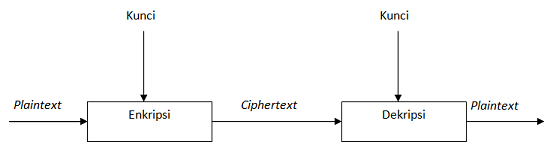
\includegraphics{gambar/kripto}
    \caption{Proses Enkripsi/Dekripsi Sederhana}
    \label{kripto}
\end{figure}

Suatu pesan yang tidak disandikan disebut sebagai \emph{plaintext} ataupun dapat disebut juga sebagai \emph{cleartext}. Proses yang dilakukan ntuk mengubah plaintext ke dalam ciphertext disebut \emph{encryption} atau \emph{encipherment}. Sedangkan proses untuk mengubah ciphertext kembali ke plaintext disebut \emph{decryprion} atau \emph{decipherment}. Secara sederhana istilah-istilah diatas dapat digambarkan pada gambar \ref{kripto}

Kriptografi adalah suatu ilmu ataupun seni mengamankan pesan, dan dilakukan oleh \emph{cryptographer}. Sedang, \emph{cryptanalys} adalah suatu ilmu dan seni membuka \emph{(breaking)} ciphertext dan orang yang melakukannya disebut \emph{cryptanalyst}.



\subsection{Enkripsi dan Dekripsi}
Proses utama dalam suatu algoritma kriptografi adalah enkripsi dan dekripsi. Enkripsi adalah proses mengamankan suatu informasi dngan membuat informasi tersebut tidak dapat dibaca tanpa bantuan pengetahuan khusus. Keuntungan dari enkripsi adalah kode asli kita tidak dapat dibaca oleh orang lain. Enkripsi mengubah sebuah plaintext ke dalam bentuk ciphertext. Pada mode ECB \emph{(Electronic Codebook)}, sebuah blok pada plaintext dienkripsi ke dalam sebuah blok ciphertext dengan panjang blok yang sama.

Dekripsi adalah proses mengembalikan suatu informasi dengan cara tertentu dan sesuai dengan algoritma enkripsi yang dipakai. Dekripsi merupakan proses kebalikan dari proses enkripsi, mengubah ciphertext kembali ke dalam bentuk plaintext. 


\subsection{Algoritma Kriptografi Klasik}
Kriptografi mempunyai sejarah yang panjang, mulai dari kriptografi Caesar yang berkembang pada zaman sebelum Masehi sampai kriptografi modern yang digunakan dalam komunikasi antar komputer di abad 20. Ada dua teknik yang paling dasar, yaitu: teknik subtitusi dan teknik transposisi.

- Teknik Subtitusi

Teknik subitusi adalah sebuah teknik enkripsi yang menggunakan metode pertukaran huruf pada dengan huruf lainnya atau dengan angka atau simbol tertentu. 

- Teknik Transposisi

Pada teknik transposisi huruf-huruf pada plaintext dan chipertext tetap sama, tetapi urutannya diubah. Dengan kata lain, teknik ini melakukan transpose terhadap rangkaian karakter di dalam teks. Nama lain untuk metode ini adalah permutasi, karena transpose setiap karakter di dalam teks sama dengan mempermutasikan karakter-karakter tersebut


\subsection{Metode Kriptografi Caesar Cipher atau Sift Chiper}
Metode kriptografi shift chiper mula-mula digunakan oleh kaisar Romawi, Julius Caesar untuk menyandikan pesan yang dikirim kepada para gubernurnya, sehingga metode ini disebut caesar chiper. Dalam kriptografi, shift chiper dikenal dengan beberapa nama seperti: code caesar atau caesar shift. 

Shift chiper merupakan teknik enkripsi yang paling sederhana dan banyak digunakan. Chiper ini berjenis chiper substitusi, dimana setiap huruf pada plaintext digantikan dengan huruf lain yang tetap pada posisi alfabet. Misalnya diketahui bahwa pergeseran = 3, maka huruf A akan digantikan oleh huruf D, huruf B menjadi huruf E, dan seterusnya. Sebagai ilustrasinya dapat dilihat pada gambar \ref{caesar}

\begin{figure}[ht!]
  \centering
    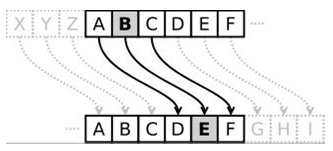
\includegraphics{gambar/caesar}
    \caption{Ilustrasi metode kriptografi Shift Chiper atau Caesar Cipher}
    \label{caesar}
\end{figure}

Transformasi shift chiper dapat direpsentasikan dengan menyelaraskan plaintext dengan chipertext ke kiri atau kanan sebanyak jumlah pergeseran yang diinginkan. Berikut ini contoh dengan jumlah pergeseran = 3. 

Plaint Alphabet 	 : ABCDEFGHIJKLMNOPQRSTUVWXYZ

Cipher Alphabet	: DEFGHIJKLMNOPQRSTUVWXYZABC

Untuk membaca pesan yang dienkripsi, penerima dapat menyelaraskan setiap huruf chipertext diterima dengan cara mencari Chiper Alpahabet dan menyelaraskan dengan plain alphabet yang ada diatasnya. Sebagai contoh dekripsinya sebagai berikut.
 
Ciphertext	: WKH TXLFN EURZQ IRA MXPSV RYHU WKH ODCB GRJ

Plaintext	 : THE QUICK BROWN FOX JUMPS OVER THE LAZY DOG


\subsection{Citra Digital}
Citra atau gambar dapat didefinisikan sebagai sebuah fungsi dua dimensi, f(x,y), dimana x dan y adalah koordinat bidang datar, dan harga fungsi f di setiap pasangan koordinat (x,y) disebut intensitas atau level keabuan \emph{(grey level)} dari gambar di titik itu.

Jika x,y dan f semuanya berhingga \emph{(finite)}, dan nilainya diskrit, maka gambarnya disebut citra digital (gambar digital).
Sebuah citra digital teridri dari sejumlah elemen yang berhingga, dimana masing-masing mempunyai lokasi dan nilai tertentu. Elemen-elemen ini disebut sebagai \emph{picture element, image element, pels} atau \emph{pixels.}

\emph{RGB Image} terkadang diaggap sebagai \emph{truecolor image}. \emph{RGB image} disimpan dalam MATLAB sebagai array nx3 yang mendefinisikan komponen warna \emph{red, green dan blue} dari masing-masing piksel. Warna dari tiap piksel ditentukan dengan kombinasi intensitas \emph{red, green dan blue} yang disimpan di tiap saluran warna di lokasi piksel tertentu. 

Format file grafik menyimpan RGB image sebaga 24-bit image, di mana komponen \emph{red, green dan blue} masing-masing 8-bit.
Suatu piksel yang mempunyai komonen warna (0,0,0) berwarna hitam, sedangkan piksel dengan komponen warna (255,255,255) berwarna putih. Tiga komponen warna untuk masing-masing piksel disimpan sebagai array tiga dimensi. 

Dasar dari pengolahan citra adalah pengolahan warna RGB pada posisi tertentu. Dalam pengolahan citra warna dipresentasikan dengan nilai hexadesimal dari 0x00000000 sampai 0x00ffffff. Warna hitam adalah 0x00000000 dan warna putih adalah 0x00ffffff. 
 Terlihat bahwa setiap warna mempunyai range nilai 00 (angka desimalnya adalah 0) dan ff (angka desimalnya adalah 255), atau mempunyai nilai derajat keabuan 256 = 28. Dengan demikian range warna yang digunakan adalah (28)(28)(28) = 224 (atau yang dikenal dengan istilah \emph{True Colour} pada Windows).
 
Nilai warna yang digunakan di atas merupakan gambungan warna cahaya merah, hijau dan biru seperti yang terlihat pada gambar \ref{rgb}. Sehingga untuk menentukan nilai dari suatu warna yang bukan warna dasar digunakan gabungan skala kecerahan dari setiap warnanya.

\begin{figure}[ht!]
  \centering
    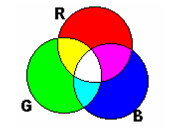
\includegraphics{gambar/rgb}
    \caption{Komposisi warna RGB}
    \label{rgb}
\end{figure}

Dari definisi diatas untuk menyajikan warna tertentu dapat dengan mudah dilakukan, yaitu dengan mencampurkan ketiga warna dasar RGB, table 1. berikut memperlihatkan contoh-contoh warna yang bisa digunakan:

\begin{figure}[ht!]
  \centering
    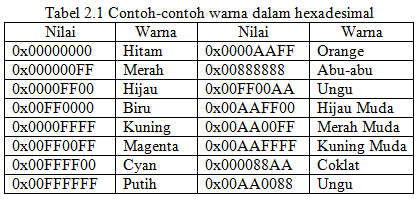
\includegraphics{gambar/tabelwarna}
    \label{tabelwarna}
\end{figure}

\subsection{Bahasa Pemrograman JAVA}
Java, dalam ilmu komputer, merupakan bahasa pemrograman berorientasi objek yang diperkenalkan pada tahun 1995 oleh Sun Microsystems, Inc., sebuah industri perangkat lunak yang cukup besar di Amerika Serikat, yang saat Java diciptakan, proyeknya dipimpin oleh James Gosling. 

Nama Java diambil karena beberapa pemrogramannya terkesan oleh keindahan pulau Jawa di Indonesia serta kenikmatan kopinya. Java memungkinkan kita membuat program-program komputer dengan paradigma yang kita jumpai di dunia nyata yang sebenarna. Paradigma yang dimaksud adalah \emph{Pemrograman Berorientasi Objek} yang dalam bahasa aslinya disebut sebagai OOP \emph{(Object Oriented Programming)}.

Salah satu alat yang dipakai untuk menulis kode bahasa pemrograman java adalah Netbeans. NetBeans merupakan sebuah proyek kode terbuka yang sukses dengan pengguna yang sangat luas, komunitas yang terus tumbuh, dan memiliki hampir 100 mitra (dan terus bertambah!). Sun Microsystems mendirikan proyek kode terbuka NetBeans pada bulan Juni 2000 dan terus menjadi sponsor utama. 

Saat ini terdapat dua produk : NetBeans IDE dan NetBeans Platform. The NetBeans IDE adalah sebuah lingkungan pengembangan  sebuah kakas untuk pemrogram menulis, mengompilasi, mencari kesalahan dan menyebarkan program. Netbeans IDE ditulis dalam Java, namun dapat mendukung bahasa pemrograman lain. Terdapat banyak modul untuk memperluas Netbeans IDE. Netbeans IDE adalah sebuah produk bebas dengan tanpa batasan bagaimana digunakan. 

Tersedia juga NetBeans Platform; sebuah fondasi yang modular dan dapat diperluas yang dapat digunakan sebagai perangkat lunak dasar untuk membuat aplikasi desktop yang besar. Mitra ISV menyediakan plug-in bernilai tambah yang dapat dengan mudah diintegrasikan ke dalam Platform dan dapat juga digunakan untuk membuat kakas dan solusi sendiri. 

Kedua produk adalah kode terbuka \emph{(open source)} dan bebas (free) untuk penggunaan komersial dan non komersial. Kode sumber tersedia untuk guna ulang dengan lisensi \emph{Common Development and Distribution License (CDDL)}.


%-------------------------------------------------------------------------------
\chapter{METODOLOGI PENELITIAN}

\section{Studi Literatur}
Tahap ini merupakan tahap awal dari sekian tahapan yang ada. Pada tahap ini penulis mengumpulkan informasi dan referensi yang berhubungan dengan kriptografi, metode caesar cipher, citra digital dan bahasa pemrograman Java beserta kompiler Netbeans.

\section{Perancangan Sistem}
Setelah melakukan studi literatur dan mengaji pustaka yang ada, maka tahap selanjutnya adalah perancangan sistem. Pada tahap ini akan dijelaskan bagaimana kerja aplikasi yang akan dibangun, sehingga sebelum aplikasi dibangun, peneliti sudah bisa mendapatkan dugaan hasil yang akan diperoleh setelah terbangunnya aplikasi ini.
 
Tujuan dari perancangan sistem adalah untuk memenuhi kebutuhan pengguna mengenai gambaran yang jelas tentang perancangan sistem yang akan dibuat serta diimplementasikan. Untuk mulai membangun suatu aplikasi kriptografi, maka penulis terlebih dahulu merencanakan alur kerja berdasarkan kebutuhan penggna yang akan menggunakan aplikasi ini. 

Adapun beberapa rancangan antarmuka pengguna, sebagai berikut:

a.	Desain Enkripsi dan Dekripsi

b.	Desain Impor File Teks (Plaintext)

c.	Desain Impor File Teks (Ciphertext)

d.	Desain Input Lokasi dan Nama Citra Berwarna

e.	Desain Ekspor Ciphertext dalam File Teks


\section{Diagram Alur Algoritma}
Berikut ini adalah diagram alur kerja aplikasi kriptografi, yang terdiri dari diagram alur proses enkripsi dan diagram alur proses dekripsi.
\begin{figure}[ht!]
  \centering
    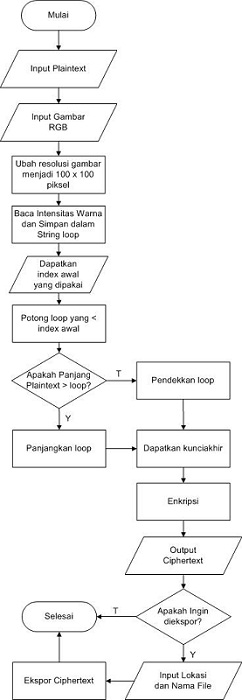
\includegraphics{gambar/Enkripsi}
    \caption{Diagram Alur Proses Enkripsi}
    \label{Enkripsi}
\end{figure}

Pada diagram alur proses enkripsi, dapat diamati bahwa:

Proses awal adalah memasukkan plainteks yang akan dienkripsi, yang mana plainteks ini dapat diketik langsung pada teks area yang telah disediakan maupun mengimpor file teks yang telah disimpan.

Tahap kedua dari proses enkripsi adalah memasukkan gambar RGB 24-bit yang akan diambil nilai intensitas warna pada setiap pikselnya. Semakin banyak variasi warna pada gambar, maka kualitas cipherteks akan lebih bagus, sebaliknya jika gambar yang diinputkan berwarna hampir sama atau sama pada setiap pikselnya, maka keamanan cipherteks akan semakin berkurang. Misalkan gambar bendera Indonesia, yang mana warna piksel pada setengah jumlah baris dan semua kolom adalah sama, yaitu merah dan putih, maka pergeseran pada setiap karakter akan sama dan hal ini akan membuat ciphertext akan mudah untuk dikenali oleh pihak yang tidak berhak.

Setelah citra digital dimasukkan, maka citra akan diubah resolusinya menjadi 100 x 100 piksel untuk membuat variasi pergeseran yang lebih unik.

Tahap selanjutnya adalah membaca nilai intensitas warna RGB yang akan dikonversi dan disusun dalam sebuah String loop. Data inilah yang nantinya akan dipakai untuk pergeseran karakter Pi+Ki.

Memasukkan index awal pada kunci akhir yang menandai awal pergeseran pada karakter pertama.

Plaintext yang diinputkan tentunya memiliki panjang yang sama atau tidak sama dengan panjang String loop yang telah dibuat. Maka tahap selanjutnya adalah atur kunci dari String loop menjadi String kunciakhir yang mana:

-	Jika panjang loop < panjang plaintext, maka kunciakhir akan diperpanjang sepanjang plaintext.

-	Selainnya panjang kunciakhir akan diperpendek sepanjang plaintext.

Setelah terbentuk kunciakhir, maka dilanjutkan dengan proses enkripsi, yang dapat dirumuskan sebagai berikut:

Ci=Pi+Ki
 
Yang mana:

Ci	= ciphertext karakter ke i

Pi	= plaintext karakter ke i

Ki	= kunciakhir karakter ke i

Pada rumusan ini tidak menggunakan modulus, hal ini dikarenakan pada bahasa pemrograman java data char hingga urutan ke-381 masih dikenali. Angka 381 didapatkan dari karakter teakhir pada keyboard standar yaitu ~ = karakter ke-126 ditambahkan dengan nilai maksimal pergeseran, yaitu intensitas warna tertinggi yang bernilai 255 pada setiap warna.

Setelah dilakukan proses enkripsi, maka akan ditampilkan sebuah cipherteks pada teks area yang disediakan. Cipherteks yang telah didapat dapat disimpan dalam file teks, jika tidak proses enkripsi berhenti sampai disini.

\begin{figure}[ht!]
  \centering
    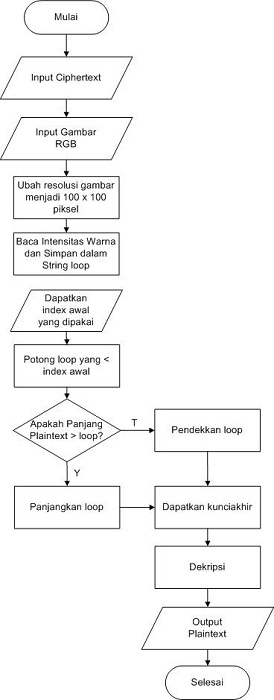
\includegraphics{gambar/dekripsi}
    \caption{Diagram Alur Proses Dekripsi}
    \label{Dekripsi}
\end{figure}

Pada diagram alur proses dekripsi, dapat diamati bahwa:

Proses awal adalah memasukkan cipherteks yang mana cipherteks ini dapat diketik pada teks area yang telah disediakan atau mengimpor file teks yang telah disimpan.

Tahap kedua dari proses dekripsi adalah memasukkan gambar RGB 24-bit yang sama dengan gambar yang digunakan saat proses enkripsi. 

Setelah citra digital dimasukkan, maka citra akan diubah resolusinya menjadi 100 x 100 piksel untuk membuat variasi pergeseran yang lebih unik.

Tahap selanjutnya adalah membaca nilai intensitas warna RGB yang akan dikonversi dan disusun dalam sebuah String loop. Data inilah yang nantinya akan dipakai untuk pergeseran karakter Pi-Ki.

Plaintext yang diinputkan tentunya memiliki panjang yang sama atau tidak sama dengan panjang String loop yang telah dibuat. Maka tahap selanjutnya adalah atur kunci dari String loop menjadi String kunciakhir yang mana:

-	Jika panjang loop < panjang plaintext, maka kunciakhir akan diperpanjang sepanjang plaintext.

-	Selainnya panjang kunciakhir akan diperpendek sepanjang plaintext.

Memasukkan index awal pada kunci akhir yang menandai awal pergeseran pada karakter pertama.

Setelah terbentuk kunciakhir, maka dilanjutkan dengan proses dekripsi, yang dapat dirumuskan sebagai berikut:

Pi=Ci-Ki
 
Yang mana:    Pi  = plaintext karakter ke i

Ci	= ciphertext karakter ke i

Ki	= kunciakhir karakter ke i

Pada rumusan ini tidak menggunakan modulus, hal ini dikarenakan pada bahasa pemrograman java data char hingga urutan ke-381 masih dikenali. Angka 381 didapatkan dari karakter teakhir pada keyboard standar yaitu ~ = karakter ke-126 ditambahkan dengan nilai maksimal pergeseran, yaitu intensitas warna tertinggi yang bernilai 255 pada setiap warna. Atau dapat disimpulkan bahwa ada batasan karakter inputan plaintext yaitu maksimal 126 dan jumlah pergeseran maksimal 255.

Setelah dilakukan proses enkripsi, maka akan ditampilkan sebuah plaintext pada teks area yang disediakan. Tahap ini adalah tahap akhir dari proses dekripsi.

\section{Metode Pengujian}
Setelah program selesai dibangun, pengujian akan dilakukan dengan menggunakan seluruh karakter input pada keyboard, selanjutnya akan diuji dengan menggunakan teks dengan panjang mulai dari 2 karakter hingga > 30.000 karakter.

Gambar yang digunakan sebagai kunci menggunakan gambar dengan format RGB 24-bit dengan resolusi mulai < 100 x 100 piksel sampai dengan resolusi > 100 x 100 piksel.

Kunci yang dipakai untuk memulai indek akan dicoba secara acak dengan catatan kurang dari 30.000.



%-----------------------------------------------------------------
%Disini akhir masukan Bab
%-----------------------------------------------------------------

%-----------------------------------------------------------------
%Disini awal masukan untuk Daftar Pustaka
%-----------------------------------------------------------------
%%\nocite{Abel2010,Guerbas201350}
%%\bibliography{research-plan}
%%\bibliographystyle{plainnat}
\begin{thebibliography}{9}

\bibitem[satu(2013)]{satu01}
Agus Kurnia, Chandra. (2014). \emph{Implementasi Kriptografi Teks Berbasis Modified Caesar Cipher Menggunakan Visual Basic}. Jember: Universitas Muhammadiyah Jember.

\bibitem[dua(2013)]{dua02}
Ariyus, Dony. (2008). \emph{Pengantar Ilmu Kriptografi Teori, Analisis, dan Implementasi}. Yogyakarta: C.V Andi Offset.

\bibitem[tiga(2013)]{tiga03}
Astuti Hermawati, Fajar. (2013). \emph{Pengolahan Citra Digital}. Yogyakarta: C.V Andi Offset.

\bibitem[empat(2013)]{empat04}
Kurnia, Chandra. (2014). \emph{Implementasi Kriptografi Teks Berbasis Modified Caesar Cipher Menggunakan Visual Basic}. Jember: Universitas Muhammadiyah Jember.

\bibitem[lima(2013)]{lima05}
Fairuzabadi, Muhammad. (2010). \emph{Implementasi Kriptografi Klasik menggunakan Borland Delphi}. Yogyakarta: Universitas PGRI Yogyakarta.

\bibitem[enam(2013)]{enam06}
Nugroho, Adi. (2008). \emph{Algoritma dan Struktur Data dalam Bahasa Java}. Yogyakarta: C.V Andi Offset.

\bibitem[tujuh(2013)]{tujuh07}
Rahardian, Rizal, dkk. (2012). \emph{Integrasi Algoritma DES pada Public Key Cryptography untuk Aplikasi Transaksi Online}. Surabaya: Politeknik Elektronika Negeri Surabaya.

\end{thebibliography}
\addcontentsline{toc}{chapter}{DAFTAR PUSTAKA}
%-----------------------------------------------------------------
%Disini akhir masukan Daftar Pustaka
%-----------------------------------------------------------------

\end{document}
